\section{Solution 1:  Metadata with Special Characters}\label{s:sol1-real}
\subsection{Metadata Storage}
This solution saves the metadata embedded with the actual data and is stored in
the column family belonging to the actual data. This means that metadata is
included in every super column in a column family as the value of column
\texttt{Metadata}. Since metadata is common for all the entities in an entity
class, every super column contains the same metadata value for this column.For
example, in the University keyspace, metadata in \texttt{Student} is stored in
every super column as seen in Figure~\ref{f:sol1-Student-md}.

In this solution, the structure of the constraints in metadata is as described
in Section~\ref{s:Metadata} and each entity class stores  its \ac{PK}
constraint and related \ac{FK} constraints in the metadata. 
The metadata stored for each column family has the following
	constraints:
	\begin{itemize}
	  \item  \ac{PK} constraint showing the primary key of the column family.
	  \item \ac{FK} constraints 
			\begin{itemize}
				\item In the case of a parent entity the \ac{FK} constraints are the \ac{FK}
				constraints of type '\texttt{F}' to identify the child entities when the entity
				is being updated or deleted.
				\item  In the case of a child entity the \ac{FK} constraint of type '\texttt{R}'
				would be stored along with the \ac{PK} constraint which indicates its parent
				entities.
				\item If an entity is both a parent and child entity, then its metadata would
				hold its \ac{PK} constraint, and the \ac{FK} constraints of both types.
			\end{itemize}
	\end{itemize}
	
For instance, \texttt{Student}  is a parent entity with a child dependendent on
it, namely \texttt{Enrolment}. 
Its metadata thus contains its \ac{PK} constraint \texttt{CONST100} and the
\ac{FK} constraint \texttt{CONST700}. Since
\texttt{Enrolment} is a child entity it  stores its \ac{PK} constraint
\texttt{CONST300} and its \ac{FK} constraints \texttt{CONST400} and
\texttt{CONST500}. Similarly, other entities like \texttt{Course} store its
\ac{PK} and respective \ac{FK} constraints.

Special characters are used within the metadata to separate the constraints and
to identify its different parts. The special characters used in this solution
are '\texttt{\{}', '\texttt{\}}','\texttt{;}' and '\texttt{:}'. Each constraint
is enclosed in curly brackets and separated from each other by the special
character '\texttt{;}'. For example, \texttt{CONST100} and \texttt{CONST700} are
enclosed in curly braces and separated by '\texttt{;}'.

	
	In every super column, the metadata is enclosed  and each
	constraint within the metadata is seprated by the special character
	'\texttt{;}'.
	
	% The first solution saves metadata as a part of every entity instance for
	% entity class and uses
	 this is
	
	

	\begin{figure}[H]
		\centering
		%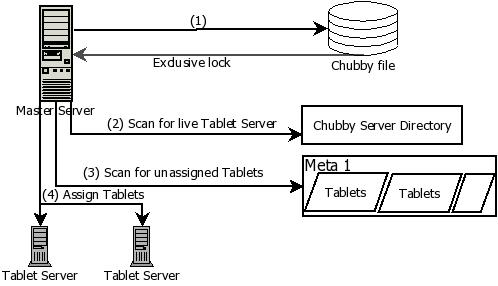
\includegraphics[width=5cm,   height=5cm]{. /figure/random. jpg}
		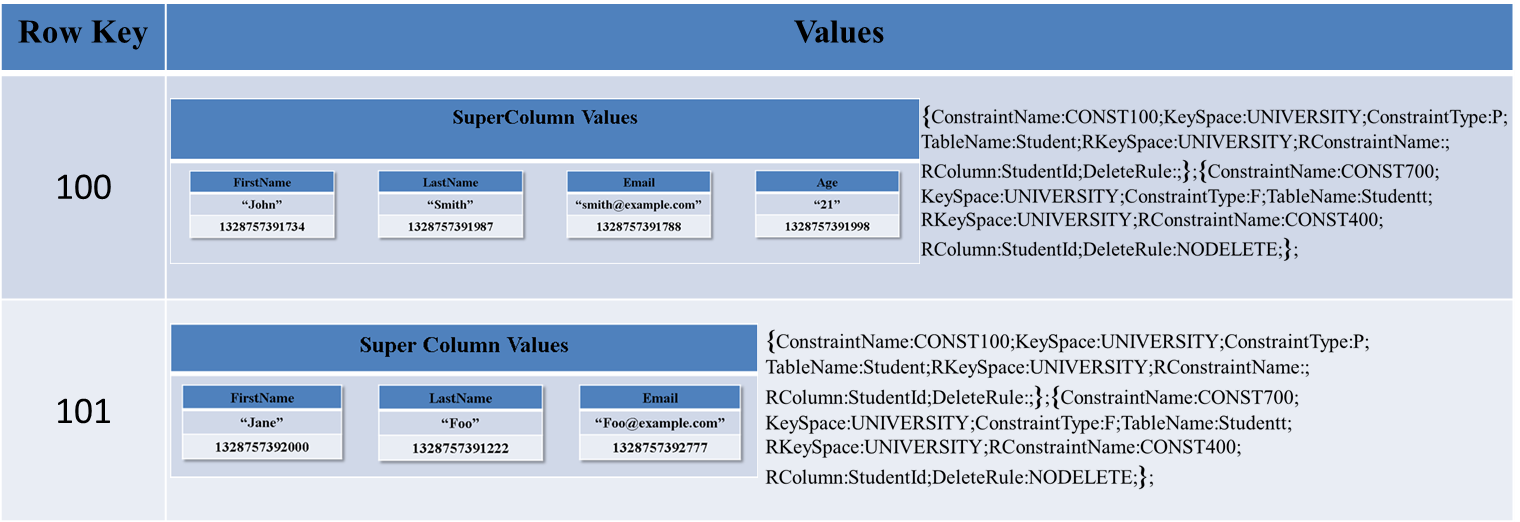
\includegraphics[width=1\textwidth]{./figure/Solutions/Solution1-Student-MD.png}
		\caption{Metadata storage in Solution 1}\label{f:sol1-Student-md}
	\end{figure}

	The metadata for a column family will contain its \ac{PK} constraint and
	\ac{FK} constraints of \texttt{} which shows the foreign keys depending on the
	primary key.
	Each constraint is surrounded by curly brackets '\texttt{\{}', '\texttt{\}}'
	and constraints are separated from each other by the special charaacter
 	'\texttt{;}'. For example, in the \texttt{Student} column family the first constraint
 	in the meetadata is the \ac{PK} constraint \texttt{CONST100}. The
	second constraint \texttt{CONST700} is separated from the \ac{PK} constraint by
	a '\texttt{;}'. The constraints following the \ac{PK} constraint indicate
	which \ac{FK} constraints are dependent on the entity.
	In this example \texttt{CONST700} shows that \texttt{CONST400} is dependent on
	it and this is necessary parent entities are updated or deleted as
	it locates its child dependencies.


	The different parts of each constraint are separated by the special character
	'\texttt{;}'. For example, a '\texttt{;}' separates the \texttt{ConstraintName}
	 and \texttt{Keyspace} and other parts in the constraints \texttt{CONST100} and
	 \texttt{CONST700}.

%|ConstraintName:CONST200;KeySpace:UNIVERSITY;ConstraintType:P;TableName:harsha_thesis_api_solution2_entity_Course;RKeySpace:UNIVERSITY;RConstraintName:;RColumn:CourseId;DeleteRule:|;
% |ConstraintName:CONST600;KeySpace:UNIVERSITY;ConstraintType:F;TableName:harsha_thesis_api_solution2_entity_Enrolment;RKeySpace:UNIVERSITY;RConstraintName:CONST500;RColumn:CourseId;DeleteRule:NODELETE|;

% 	For this solution,  the different parts of the metadata is
% 	accessed by the \texttt{ValidationHandler}  to determine whether the entity has
% 	any dependencies.
	Each part and its value are separated by the special character
	'\texttt{:}'. For example, \texttt{ConstraintName} is separated from
	its value \texttt{CONST100} with a \texttt{:}. This helps in identifying the
	constraint part name  and the values while parsing the metadata information
	in the \ac{API}.
\subsection{Metadata Retrieval}
	The different parts of the metadata is parsed by the
	\texttt{BaseEntity} where each constraint in the metadata is handled as a
	\texttt{String}. In this example, the whole of \texttt{CONST100} is
	considered as one \texttt{String}. All the special characters used within the
	metadata become the delimiters for parsing the \texttt{String} and splitting it
	into tokens.
	The delimiters used for parsing are:
	\begin{itemize}
	  \item Special characters '\texttt{\{}', '\texttt{\}}' and '\texttt{;}' are
	  the delimiters for extracting each constraint formt he metedata.
	  \item Special character '\texttt{;}' is the delimiter for identifying each
	  part within a constraint.
	  \item Special character '\texttt{:}' is the delimiter for extracting the
	  field name and the value from each part of the constraint.
	\end{itemize}

	The steps involved in the parsing are:

	Thus, each of these tokens would hold one of the parts of the constraint. For
	example, the metadata for \texttt{Student} entity will be parsed into tokens
	where one token will contain the value of \texttt{ConstraintName}
	\texttt{CONST100}, while another will contain the \texttt{Keyspace} value
	\texttt{UNIVERSITY} and likewise all the parts of the constraint will be
	tokenised. Thus, the \texttt{ValidationHandler} accesses the tokens to determine
	the various parts fo the metadata. For example, to determine the
	\texttt{DeleteRule} for a \ac{FK} constraint the \texttt{ValidationHandler}
	would read the respective token.

	The logic for the referential integrity validation by the
	\texttt{ValidationHandler} once the \texttt{String} metedata is parsed is the
	same as described in Section~\ref{ss:VH}.

	In this solution, the metadata is saved  when entities are inserted into the
	column family and thus the metadata is a part of each of the entity.  Since the
	metadata is present as the value in every super column,  accessing the metadata
	information for referential integrity validation is as simple as accessing the
	value itself,  requiring no additional actions or connection to the
	keyspace. Saving the metadata as embedded metadata in this solution is useful
	as entities are replicated across the distributed cluster, making metadata
	easily accessible by every node in the cluster, since it is a part of the
	entity.

	The \ac{API} parses the metadata of an entity by reading any of its
	instances and need not load metadata from any external location.

	On the other hand,  the metadata for an entity would be the same for all its
	instances .  For example,  in the University example,  the metadata
	information for the \texttt{Student} entity is applicable to each of its
	instances,  indicating that each instance  should have a primary key called
	\texttt{StudentID}.
	Similarly,  all \texttt{Course} instances have the same \ac{PK} constraints
	applied on it.  When metadata is saved as a part of the  value,
	every instance of an entity will contain the constraint information
	in it's value.  Since the metadata information and constraints are same for all
	the instances of a single entity ,  this metadata is repeated every time an
	instance of the entity is inserted.  For example,  if
	\texttt{1000} \texttt{Student} instances are inserted,  the metadata for these
	\texttt{1000} instances are saved \texttt{1000} times too, along with these
	instances.  But the metadata is exactly same for all the
	instances \todo{(Figure~\ref{})}.


	The distributed nature of cloud \ac{NoSQL} \acp{DBMS} also means that the
	metadata is not only repeated several times within the same column family,  but
	also across the nodes in the cluster, thus increasing the redundancy of
	the metadata.  But such a redundancy and consumption
	of space to store the metadata is not a potential issue
	in cloud column-oriented key-value \acp{DBMS}, since storage on the cloud is
	inexpensive and  does not affect the economic benefits.

	Such a storage mechanism is not expected to affect the efficiency of the
	cluster negatively as the metadata information is not large in size and is
	easily replicated along with the actual data and does not exert any extra
	resources in the cluster.  The performance of this solution is analysed  in
	Chapter~\ref{}.

	Much research has been done in the area of  metadata management in distributed
	environments,  where emphasis is laid on the synchronous updates of metadata
	storage as well as its efficient storage and access mechanisms(\todo{cite more}
	Hackl et al.  2010).
	In Hackl et al.  (2010),  metadata management is discussed in the context of
	huge file systems, where metadata is stored separately in a suitable \ac{DBMS}
	so that such file systems can be managed and administered efficiently without
	slowing them down.  To analyse which type of \ac{DBMS} was more suitable for such a
	metadata storage,  they conducted various experiments and concluded that
	key-value \acp{DBMS} were more efficient in terms of speed,  memory and resource
	consumption when compared to popular \acp{RDBMS}.  As a part of their
	experiments, they adopted an interesting approach to store metadata in a
	key-value \ac{DBMS} ,  namely Tokyo Cabinet,  a popular \ac{NoSQL} \ac{DBMS}
	that stores records as simple key-value pairs in data files. Unlike Cassandra,
	tokyoCabinet does not involve data types or columns
	and so on (\todo{cite}).  In their approach,  metadata about the file system
	used in their experiment is inserted as a value which is associated with a unique key and the
	different parts of the metadata are separated by semicolons (Hackl et al.  2010).
	